\documentclass{article}
\usepackage[top=1in,left=1in,right=1in,bottom=1in]{geometry}
\usepackage{graphicx}
\usepackage{hyperref}
\usepackage{pdfpages}
\title{github for SNO+ Code}
\author{Andy Mastbaum\footnote{\href{mailto:mastbaum@hep.upenn.edu}{mastbaum@hep.upenn.edu}}}
\date{SNO+ Code Integrity Committee}
\begin{document}
\maketitle
\tableofcontents
\section{Introduction}
In February 2012, the SNO+ code repository moved from an SVN repository hosted at SNOLAB to a git repository hosted by \href{http://github.com}{github.com}. The transition was proposed by the Code Integrity Committee in November 2011 and approved by the SNO+ board in January 2012.

Using git and github makes it easier to share code and allows review to happen before code is committed to the main repository, ensuring that a high-quality code base is always available to collaborators. This document briefly outlines the motivations for the transition, explains the differences between git and SVN, and provides a walk-through of typical developer workflow. A ``cheat sheet'' suitable for hanging near a computer is attached at the end.
\subsection{What is git?}
\href{http://git-scm.com}{git} is a distributed version control system, originally developed by Linus Torvalds and used for Linux kernel development. Now, it is used by such prominent projects as Perl, Gnome, Android, X11, and SNO+ RAT.

Distributed version control systems (DCVS) are next-generation version control systems (VCS) structured with a network of peer repositories, rather than a single ``master'' repository. In SVN, a regular VCS, users ``check out'' a snapshot of a repository, make changes, and push the new snapshot to the master repository every time they wish to change something. In git, a DCVS, users ``clone'' a repository, creating a complete replica of it on the user's computer. The user can commit to this repository at will, view the commit history and ``check out'' any past revision offline, and later push their changes back to the parent.

The key advantage to a DCVS is distributed development -- many developers working on parts of project simultaneously.
\subsection{What is github?}
\href{http://www.github.com}{github} is a git repository hosting service that offers a suite of best-in-class source code management tools. github encourages ``forking'' of projects for collaborative development. In the past, forking meant divergence: a group of developers broke off from the project to pursue different direction. Now, thanks to git's distributed nature, forking means collaboration: you see a project that needs help, fork it, make changes, and give those changes back to the original repository. github makes this process as easy as a few clicks.

The most important github feature for SNO+ is the Pull Request system, the mechanism by which developers ``give those changes back'' from a fork to the parent repository. Pull Requests provide a chance for code to be reviewed, discussed, and improved before it is committed to the main RAT repository.

github also offers advanced project management tools, including an excellent bug tracking system that integrates with release management, which replace and improve upon the tools in Trac.
\section{User's Guide}
This section explains what to do if you want to {\it use} RAT, but not make changes (yet). If you plan to {\it develop} new features for RAT, skip ahead to Section \ref{devguide}.
\subsection{Getting started with github}
\label{get-started}
Before you can see the code, you'll need to be added as a member of the SNO+ organization on github, \href{http://github.com/snoplus}{snoplus}.
\begin{enumerate}
\item Make yourself a free account here: \href{https://github.com/signup/free}{https://github.com/signup/free}
\item Send a message to the CIC (\href{mailto:snopluscode@snolab.ca}{snopluscode@snolab.ca}) asking to be added to the SNO+ organization
\item Once you've been added, you should be able to see the private repositories at \href{http://github.com/snoplus}{github.com/snoplus}.
\end{enumerate}

\subsection{Getting the code}
Like with SVN, getting RAT is a one-liner:
\begin{verbatim}
  $ git clone git@github.com:snoplus/rat.git
\end{verbatim}
This puts RAT in a new directory called {\tt rat}. To put it somewhere else, tack the destination directory name on the end of that line.

The documentation is in a separate repository. To get the documentation, run:
\begin{verbatim}
  $ git clone git@github.com:snoplus/rat-doc.git
\end{verbatim}

Viewable documentation, re-built after every change, is available \href{http://ratbuild.hep.upenn.edu/snoplus/doc}{here}.

You can think of {\tt git clone} as similar to {\tt svn co}, but there is an important difference: you are getting the entire repository, history and all.

\subsection{Checking out an old revision}
You already have the entire history on your computer, so you can check out any revision even while on a plane! Run {\tt git checkout} to get to another revision:
\begin{verbatim}
  $ git checkout [revision id]
\end{verbatim}
After running {\tt git checkout}, your directory is magically transformed into the revision you asked for.\\

{\bf Because the history of a git repository doesn't have to be linear, revisions can't be named with a sequential number.} Find a revision ID by:
\begin{itemize}
\item Searching the history on github: \href{https://github.com/snoplus/rat/search}{https://github.com/snoplus/rat/search}. To find an old commit, try searching for the SVN revision number (no ``r'') in commit messages.
\item Looking at the history on github.com: \href{https://github.com/snoplus/rat/commits/master}{https://github.com/snoplus/rat/commits/master}
\item Looking at the history by running {\tt git log}
\end{itemize}

Anywhere you can use a revision ID, you can also use special identifiers like {\tt HEAD} (the most recent commit) or any tag name (e.g. {\tt release-0.00}).

\subsection{Becoming a developer later}
If you followed the steps above but now wish to start contributing code, do not fret.
\begin{enumerate}
\item Create your own fork of RAT, following the steps in Section \ref{create-fork}
\item Tell your local repo about your fork (you can call it anything you want):
\begin{verbatim}
  $ git remote rename origin snoplus
  $ git remote add origin git@github.com:[your-username]/rat.git
\end{verbatim}
\item You can now push commits to your fork using {\tt git push} and pull changes from the main SNO+ repository using {\tt git pull snoplus}. See Section \ref{patterns} for what to do next.
\end{enumerate}

\section{Developer's Guide}
\label{devguide}
This sections explains how to change or contribute code. If you haven't already, get set up with an account as described in Section \ref{get-started}.
\subsection{Create a fork}
\label{create-fork}
The first step is to create a fork of the main RAT repository. Your fork is a duplicate of the main repository which you can work on in isolation, even doing your own project management with bug tickets and milestones. When you're ready, you can send a Pull Request, asking to have your changes merged into the main repository. Typically you will make many commits, incrementally working toward a new feature, between Pull Requests. This helps you keep track of every step, and eliminates ``code bombs'' that plague SVN projects.

Your fork is a proper repository unto itself. Other people can fork it, make changes, and send {\it you} Pull Requests, which you can review and accept, then pass them along as part of a Pull Request to the main RAT repository. The collaborative possibilities are endless, and in every case, git keeps track of all the history of who changed what, when, and why.\\

{\bf To fork a repository (be it RAT, the documentation, or any other), navigate there on github, and click the "Fork" button in the upper right corner.} Done.\\

Your fork will appear in your list of repositories on your github page (github.com/[your-username]).

\subsection{Clone Your fork}
\label{clone-fork}
You now need to clone your fork onto your computer so that you can get coding. If you forked RAT, for example:
\begin{verbatim}
  $ git clone git@github.com:[your-username]/rat.git
\end{verbatim}
This puts RAT in a new directory called {\tt rat}. To put it somewhere else, tack the destination directory name on the end of that line.\\

The URL you need to {\tt git clone} to clone a repository always appears at the top of that repository's page on github.

\subsection{Development Patterns}
\label{patterns}
Since you are working on your own repository, you needn't feel shy about committing often. The code doesn't need to be polished until it's time to send a Pull Request. The commands checking the status of your work are quite similar to SVN's:
\begin{description}
\item[{\tt git status}] Shows which files have been modified, added, and removed
\item[{\tt git diff}] Shows a summary of all changes since the last commit
\end{description}

\subsubsection{Committing Changes}
To commit changes, run  {\tt git commit -a}.\\

{\bf This differs from SVN in a very important way: your local copy is a repository, and must be synchronized with the one on github. Commits alone never leave your computer.}\\

To push your changes to your fork on github, run {\tt git push}. You don't need to do this after every commit, but push often.\\

{\tt git commit -a} commits {\it all} the outstanding changes shown by {\tt git status}. To instead commit individual files, use {\tt git commit file1 [file2 ...]}.\\

{\tt git commit} will pop open your system's default editor so you can enter a commit message. To change the editor, set the {\tt EDITOR} environment variable, e.g. {\tt \$ export EDITOR=vim}. For a short message, you can also do {\tt \$ git commit -am "message here"}.

\subsubsection{Branches}
Branches are very easy to create and use in git:
\begin{description}
\item[{\tt git branch}] List all branches
\item[{\tt git branch [branch-name]}] Make a new branch
\item[{\tt git branch -D [branch-name]}] Delete a branch
\item[{\tt git checkout [branch-name]}] Switch to another branch
\item[{\tt git merge [branch-name]}] Merge changes from another branch onto your current one
\item[{\tt git push origin [branch-name]}] Push a branch into the remote repository named ``origin'' (push doesn't do this by default)
\end{description}
Branches are great for playing around with new ideas or working on code you don't want messing up the main development path.

\subsubsection{Continuous Integration}
``Continuous Integration'' refers to coding practices where code quality is checked as often as possible. In keeping with this philosophy, the \href{http://ratbuild.hep.upenn.edu/snoplus/build}{automatic build testing system} tests every push to the main RAT repository. Developers are encouraged to use the {\tt ratci} tool packaged with RAT to run build tests often, as well. To run a build test on your fork, simply run {\tt ratci -m "message"}.

Another CI tip that will make everyone's life easier is to synchronize your fork with the main RAT repository very often (daily). It is much easier to resolve a few small conflicts as they arise than to try to merge a huge set of commits littered with conflicting code.

To keep your fork up to date, you can pull down changes from the main RAT repository. First, you first have to tell git where this is: {\tt \$ git remote add snoplus git@github.com:snoplus/rat}. You only need to do this once.

Then, to pull in changes (approximately daily):
\begin{verbatim}
  $ git fetch snoplus         # grab snoplus/rat from github
  $ git merge snoplus/master  # merge snoplus/rat's master branch into yours
\end{verbatim}
git will automatically resolve conflicts if possible. If there are any conflicts it can't handle, it will ask you what to do. Once it's all merged, run {\tt git push} to ship it off to github.\\

There is another command {\tt git pull} which does {\tt fetch} then {\tt merge}, which is best used when you know there aren't any conflicts (i.e. you have no outstanding changes).

\subsection{Get Your Changes into the Main RAT Repository}
At last, the feature is done, the bug is fixed, the document is documented; you're ready to push your changes off into the main snoplus repository. First, consider:
\begin{itemize}
\item Is the change appropriately documented?
\item Does the code comply with the \href{https://www.snolab.ca/snoplus/private/DocDB/cgi/ShowDocument?docid=1018}{Style Guide and Coding Conventions}?
\item Have any relevant {\tt rattests}s been updated?
\item Has it passed a build test (using {\tt ratci})?
\end{itemize}

To send off your changes, click the ``Pull Request'' button at the upper right corner of your fork's repository page on github. On the Pull Request page, you can review your changes (as commits and the overall diff), and can optionally change which commits are included. In most cases, defaults are fine -- just enter a title and description describing your changes and click ``Send pull request.'' If you're working on RAT, please include in your request a link to successful {\tt ratci} results.\\

This will notify an administrator of the snoplus repository, who will take a look over the changes. If anything's amiss, such as missing documentation, the reviewer will make a comment, and you can add commits to address any issues. The pull request page becomes a conversation about the changes, where people can make comments on individual commits, lines, or blocks of code, eliminating the cumbersome review-via-email process.

\section{git and github Resources}
A few of the great resources for getting acquainted with git:
\begin{description}
\item[github Bootcamp] \href{http://help.github.com}{help.github.com}
\item[git Cheat Sheets] \href{http://help.github.com/git-cheat-sheets}{help.github.com/git-cheat-sheets}
\item[Complete git command reference] \href{http://gitref.org}{gitref.org}
\item[{\tt git help}] git is very well-documented -- try, e.g. {\tt git help branch}.
\end{description}

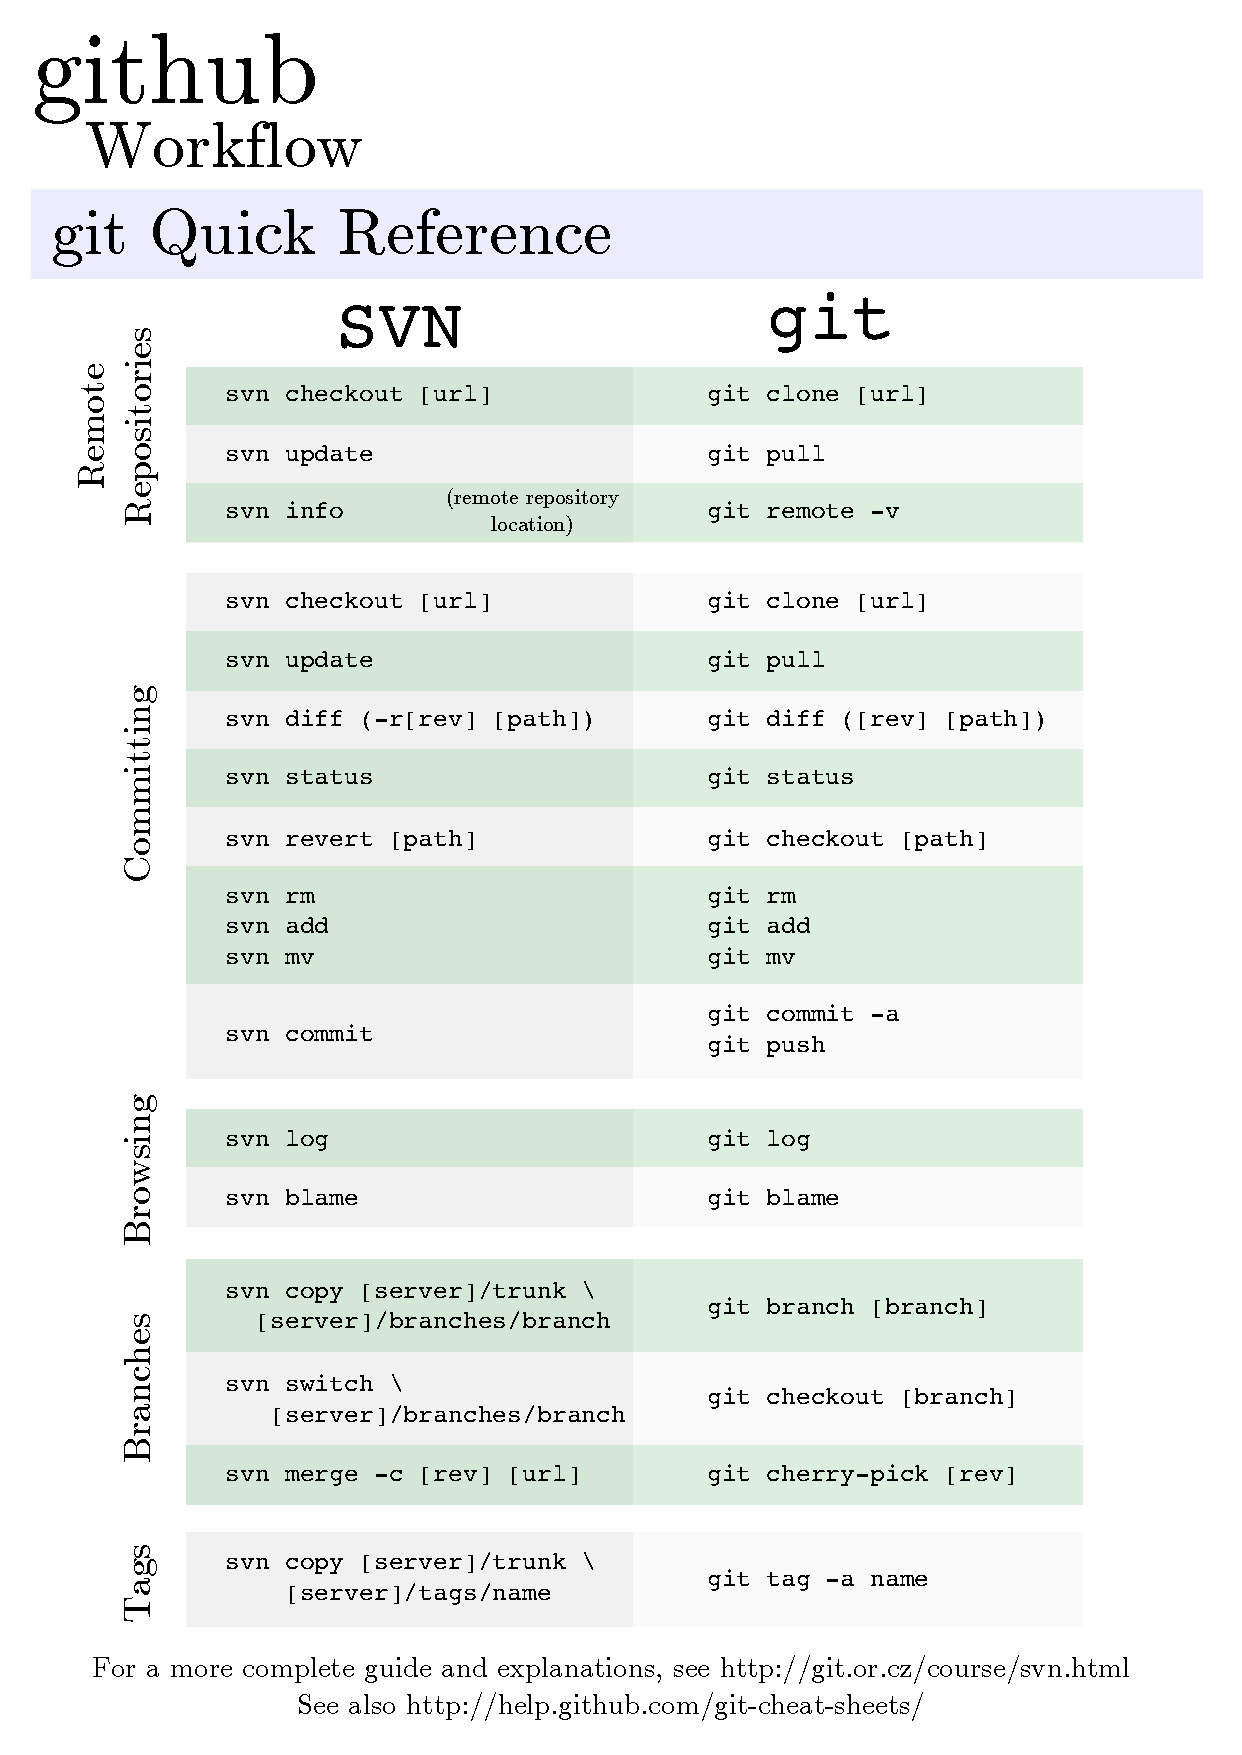
\includepdf[addtotoc={6,5,1,git Cheat Sheet,cheat-sheet}]{../illustrated/cheatsheet.pdf}

\end{document}

